\section{Resultados}
\begin{frame}{Resultados}

Una vez construidos los componentes que forman el branch and cut, pasamos a evaluar su performance compar�ndolo contra otros algoritmos de programaci�n lineal entera ya existentes.

\end{frame}

\subsection{Conjunto de prueba}
\begin{frame}{Conjunto de prueba}

La mayor�a de las pruebas fueron ejecutadas sobre dos familias de grafos aleatorios: 
\begin{itemize}
\item{Grafos binomiales}
\item{Grafos de Holme-Kim}
\end{itemize}
\vskip 10pt
Asimismo se hicieron pruebas sobre grafos del conjunto de instancias \textsc{dimacs} para coloreo.

\end{frame}

\begin{frame}{Grafos binomiales}

Para cada par de nodos en el grafo, se construye un eje uni�ndolos con probabilidad uniforme $p$. Las particiones se construyen agrupando a los nodos de manera aleatoria.

\begin{figure}
  \begin{center}
    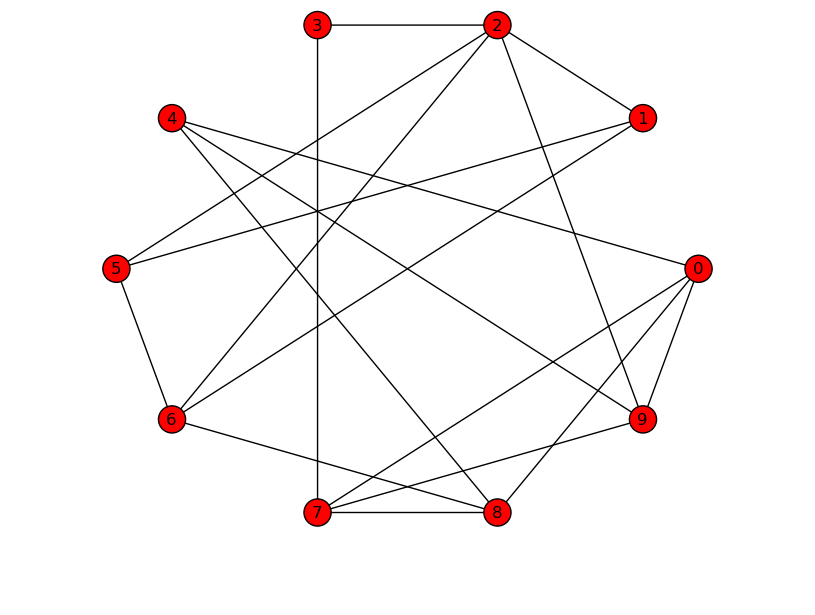
\includegraphics[scale=0.3]{binomial-10-04.png}
  \end{center}
\end{figure}

\end{frame}

\begin{frame}{Grafos de Holme-Kim}

Los nodos se agregan iterativamente, cada nuevo nodo debe ser adyacente a una cantidad $m$ de nodos ya existentes, con preferencia hacia los de mayor grado, y con cierta probabilidad de agregar un eje extra formando un tri�ngulo; las particiones se construyen igual que en el caso anterior.

\begin{figure}
  \begin{center}
    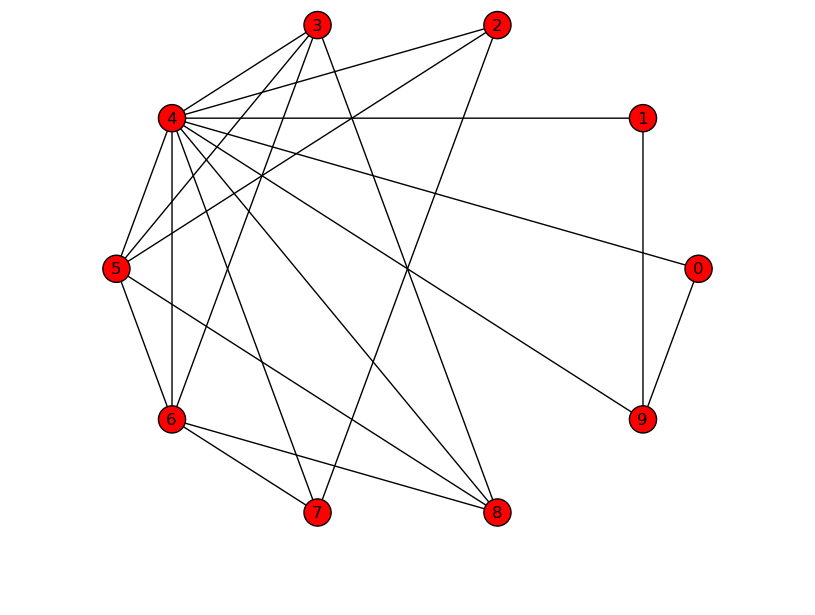
\includegraphics[scale=0.3]{hk-10-04.png}
  \end{center}
\end{figure}

\end{frame}

\begin{frame}{Instancias DIMACS}

Los grafos correspondientes a las challenges de DIMACS son grafos particularmente dif�ciles de colorear. Construimos a partir de ellos grafos particionados agrupando los nodos de manera aleatoria.

\begin{figure}
  \begin{center}
    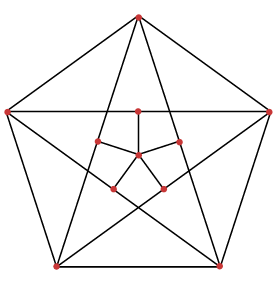
\includegraphics[scale=0.3]{mycielski.png}
  \end{center}
\end{figure}

\end{frame}

\subsection{Versus Cplex}
\begin{frame}{Resultados en binomiales PCP vs Cplex}

Ejecutamos el branch and cut sobre grafos aleatorios binomiales, de $90$ nodos y $2$ nodos por partici�n. Todos los grafos de baja densidad fueron resueltos a optimalidad, en distintos tiempos:

\includechart{chartbncdenstime.png}

\end{frame}

\begin{frame}{Resultados en binomiales PCP vs Cplex}

Los de mayor densidad, obtuvieron los siguientes gaps en promedio tras 2hs de ejecuci�n:

\includechart{chartbncdens.png}

\end{frame}

\begin{frame}{Tama�os de partici�n PCP vs Cplex}

Evaluamos tambi�n c�mo cambia la performance de los algoritmos conforme var�a el tama�o de partici�n. Para tama�os de $1$ a $3$ nodos por partici�n, en binomiales de $90$ nodos y densidad $60\%$, obtuvimos:

\includechart{chartbncpartsmall.png}

\end{frame}

\begin{frame}{Tama�os de partici�n PCP vs Cplex}

Los grafos de particiones de mayor tama�o fueron todos resueltos a optimalidad, con los siguientes tiempos:

\includechart{chartbncpartlarge.png}

\end{frame}

\begin{frame}{Instancias \textsc{Dimacs} PCP vs Cplex}

Particionando de forma aleatoria $15$ instancias \textsc{Dimacs} diferentes, los resultados obtenidos fueron:

\begin{align*}
\text{Mejor resultado PCP:}\quad & 4/15 \\
\text{Mejor resultado Cplex:}\quad & 4/15 \\
\text{Empates:}\quad & 7/15 \\
\end{align*}

\end{frame}

\subsection{Versus Representatives Model}
\begin{frame}{Representatives Model}

Comparamos nuestro algoritmo contra el derivado del \textit{representatives model}, un modelo alternativo para coloreo, el cual tambi�n fue generalizado a coloreo particionado y llevado a un branch and cut.
\vskip 10pt
En este modelo, cada nodo es \textit{representado} por otro (o por s� mismo). Todos los nodos que tienen el mismo representante, pertenecen a una misma clase de equivalencia y utilizan el mismo color.

\[
x_{uv} \quad \text{1 sii el nodo $u$ representa al nodo $v$}
\]

\end{frame}

\begin{frame}{PCP vs Representatives Model}

Dados grafos aleatorios de $90$ nodos, particiones de $2$ nodos y distinta densidad, comparamos qu� porcentaje de las instancias evaluadas fueron resueltas a optimalidad por ambos algoritmos tras $2$ horas de ejecuci�n.

\includechart{chartbncrepr.png}

\end{frame}